\section{Introduction}
The deformability, adaptiveness, and compliance of invertebrates serve as an inspiration for continuum soft robots.
While serial continuum soft robots have been intensively investigated in recent years~\cite{della2023model}, parallel soft robots~\cite{hughes2020extensible} % more references for parallel robots: zhang2020modeling
are less studied despite exhibiting exciting properties such as an improved stiffness-to-weight ratio. 
One recent development in this field is robots based on \glspl{HSA}~\cite{truby2021recipe, kaarthik2022motorized, stolzle2024guiding} in which multiple \gls{HSA} rods are connected at their distal end through a rigid platform. 
Twisting of the proximal end of an \gls{HSA} % with an electric actuator 
causes the rod to elongate 
% Differential electric actuation of the HSA robot 
and enables complex motion primitives in 3D space.
Recent work has investigated 
% proprioception~\cite{zhang2022vision}, 
the mechanical characterization~\cite{good2022expanding}, simulation~\cite{stolzle2023modelling}, and kinematic modeling~\cite{garg2022kinematic, stolzle2023modelling} of \gls{HSA} robots but control has yet to be tackled.
% Still, the task of control is still unsolved as \textcolor{orange}{prior work} and solutions need to be developed on how to deal with the challenges of underactuation and changing stiffness properties. 
In this work, we make a first step towards achieving task-space control by designing model-based regulators for planar motions. Our approach considers essential characteristics of \gls{HSA} robots, such as underactuation, shear strains, and varying stiffness. % and thus can serve as a building block for future research.

\begin{figure}[ht]
    \centering
    \subfigure[Blockscheme]{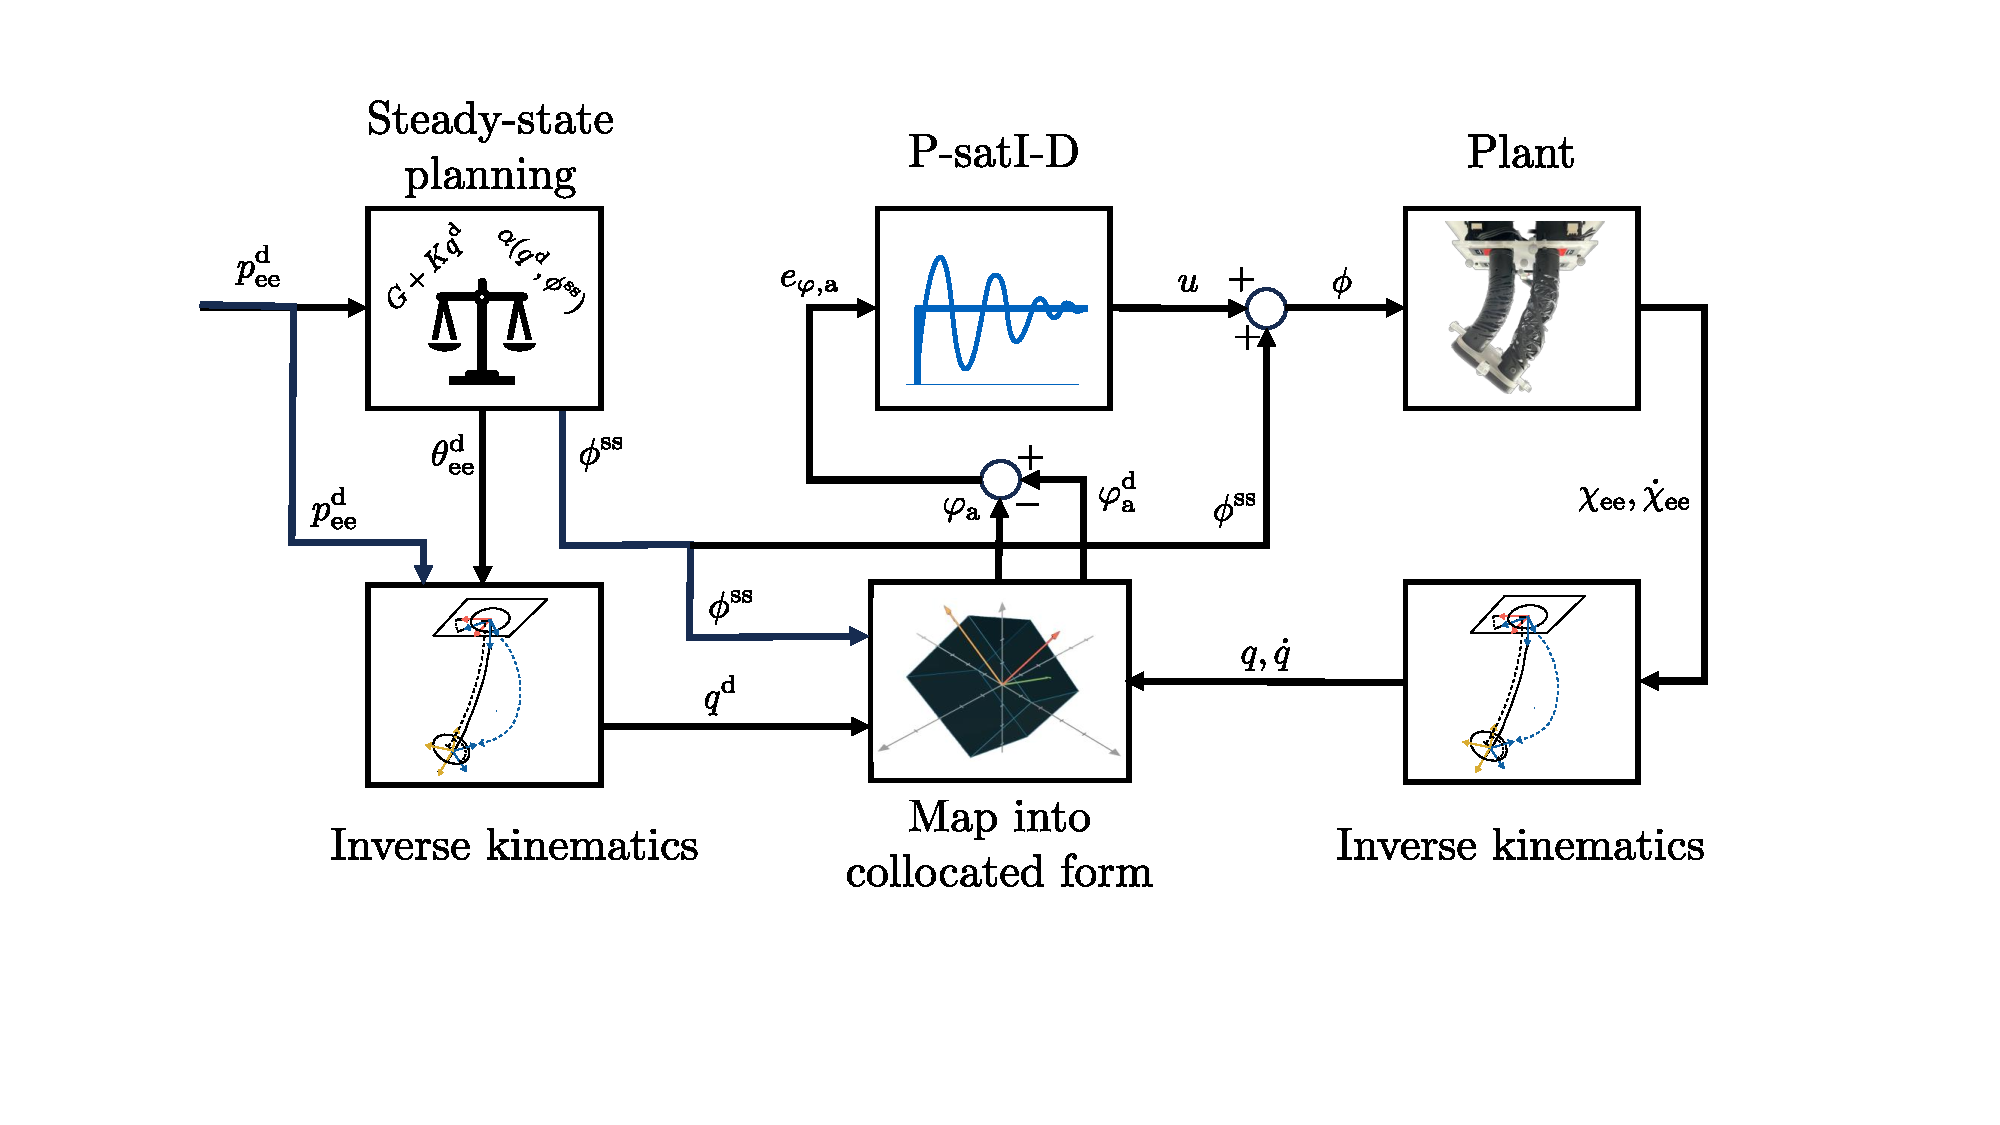
\includegraphics[width=0.62\textwidth]{hsacontrol/figures/control_scheme/control_scheme_v4_cropped.pdf}\label{fig:hsacontrol:block_scheme_closed_loop_control}}
    \subfigure[Operational workspace]{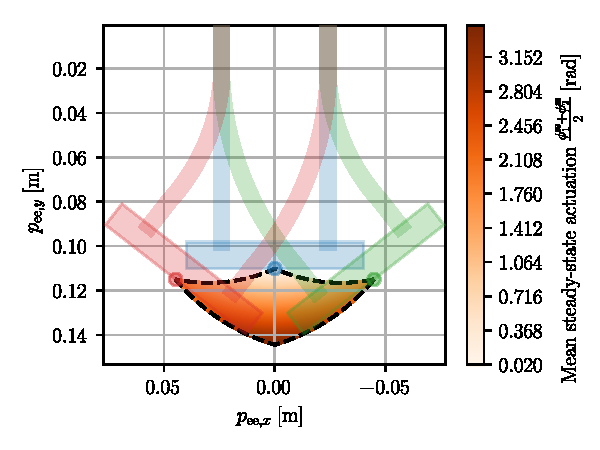
\includegraphics[width=0.37\columnwidth, trim={7, 7, 7, 7}]{hsacontrol/figures/kinematics/fpu_operational_workspace.pdf}\label{fig:hsacontrol:kinematics:workspace}}
    \caption{\textbf{Panel (a):} Block scheme of the closed-loop system: we plan the steady-state behavior such that the end-effector matches the given desired position $p_\mathrm{ee}^\mathrm{d}$. The outputs of this planning are the steady-state actuation $\phi^\mathrm{ss}$ and a suitable end-effector orientation $\theta_\mathrm{ee}^\mathrm{d}$. After leveraging inverse kinematics to identify the desired and current configuration, $q$ is mapped into a collocated form where the inputs are decoupled. Finally, we use a P-satI-D feedback controller on the actuation coordinates $\varphi$. \textbf{Panel (b):} Visualization of the operational workspace of a planar HSA robot consisting of FPU rods. The colored area within the black dashed borders represents the positions the end-effector (visualized as a dot) can reach. The coloring denotes the mean magnitude of actuation (i.e., twisting of the rods). Furthermore, we plot three sample configurations: the unactuated straight configuration $q = [0, 0, 0]^\mathrm{T}$ (blue), maximum clockwise bending $q = [\SI{-11.2}{rad \per m}, 0.08, 0.30]^\mathrm{T}$ (red), and maximum counter-clockwise bending $q = [\SI{11.2}{rad \per m}, -0.08, 0.30]^\mathrm{T}$ (green).}
\end{figure}

\textcolor{red}{TODO: make connection to HSA model chapter}
We notice that the resulting planar dynamics are underactuated
%  as prior work has shown that shear cannot be neglected~\cite{stolzle2023modelling} 
and that the actuation forces are non-affine with respect to the control inputs, which are the motor angles. The latter is a peculiarity of these systems, rarely observed in other robots.
Based on the model knowledge, we devise a control strategy shown in Fig.~\ref{fig:hsacontrol:block_scheme_closed_loop_control} that first maps end-effector positions to desired configurations and steady-state (feedforward) control inputs and then 
% in addition  to this static compensation of gravitational and elastic forces 
also applies a P-satI-D~\cite{pustina2022p} feedback action on the collocated form~\cite{pustina2024input} of the system dynamics.

In summary, we state our contributions as (i) the derivation of a planar HSA dynamic model in collocated form, (ii) a provably stable model-based control strategy for guiding the end-effector of the robot towards a desired position in Cartesian space, and (iii) experimental verification of both the model and the controller. A video accompanies this chapter explaining the methodology and displaying video recordings of the control experiments\footnote{\url{https://youtu.be/7PgKnE_MOsY}}.


%Structure
%\begin{enumerate}
%    \item Why soft robots
%    % \item Parallel soft robots have not been widely tested out,  have interesting characteristics such as higher bending stiffness with low weight
%    \item HSAs have this special mechanism in which the motors acts throught he stiffness of the hsa on the robot shape
%    \item Control has only been performed with PID, no model-based control. Problem of underactuation needs to be solved. Way to deal with changing stiffness characteristics
%\end{enumerate}
%
%Our contributions
%\begin{itemize}
%    \item Closed-form inverse kinematics for planar continuum robots modelled using PCS
%    \item An Euler-Lagrangian model for the dynamics of HSA robots, which is then also verified experimentally 
%    \item Proposal of a control strategy involving mapping from task-space to configuration-space and PID controller respecting the underactuation
%    \item Experiments involving Model-based regulation of HSA robots
%\end{itemize}